\documentclass[11pt]{article}

\usepackage{extramarks}
\usepackage{listings}
\usepackage{graphicx}
\graphicspath{ {img/} }

\title{\textbf{AITF Implementation Design Document}}
\author{Nick Muesch, Nick Kalamvokis, Ted Meyer}
\date{}
\begin{document}

\maketitle

\section{Network Design}

In Figure 1 H is an honest party participating in AITF, V is the victim, A is the attacker, and I is an internet backbone router. Ag, Hg, and Vg are the respective gateways for each of the Attacker, Honest party, and Victim. 
\begin{figure}[h!]
  \caption{non-trivial network design}
  \centering
    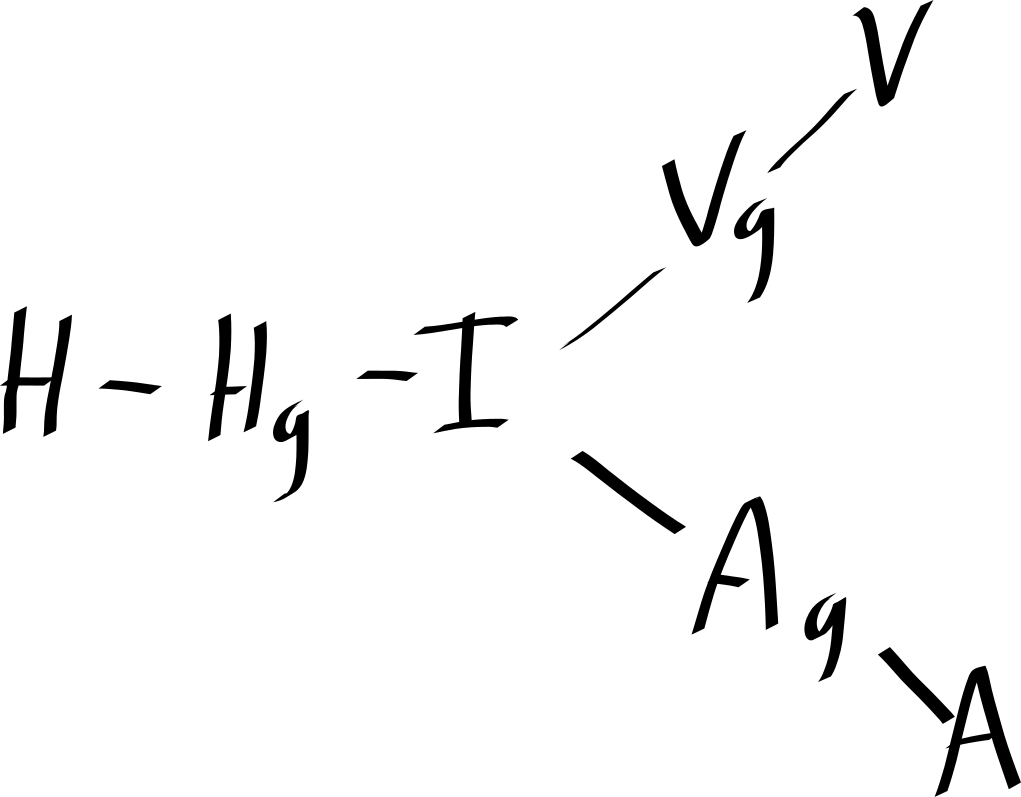
\includegraphics[width=0.5\textwidth]{network}
\end{figure}
In this scenario, we assume that all gateways and their clients are AITF enabled. While this would of course break backwards compatibility with the current architecture of the internet, we feel that it is outside the scope of the project to attempt a backwards compatible system. A more advanced description of the network protocol will be described later when discussing security and vulnerabilities of the AITF protocol.

\newpage

\section{Packet and Header Design}
The core component of the AITF system is the shim layer that will be inserted between the IP header and the IP payload. In keeping with the style of RFC 791 for internet packet headers, the shim layer is specified as such:

\texttt {
	\lstinputlisting[basicstyle=\ttfamily\scriptsize]{ip_spec.txt}
}

Based on the statistics and calculations in the [original paper], we concluded that a minimum of six bytes are needed in order to maintain an uncrackable key. However, six is not a very nice number (read: not a power of two), so eight bytes were used instead. The shim layer is treated as a stack; each AITF enabled router that sees any type of packet will do four things: 
\begin{enumerate}
	\item The router will change the protocol ID in the original IP header to 254. This ID is reserved by RFC 791 for research use.
	\item The router will increment the shim size field in the options buffer in the IP header
	\item The router will write the IP address of its outgoing connection and the randomly generated number, which is keyed on the destination IP of the original IP header.
	\item The router will write the remainder of the packet
\end{enumerate}
Clients such as V, H, and A will also strip the AITF shim layer by calculating its size from the options header. This information will have to be stored in a key-value pair structure, such that paths can be retrieved by source IP on request.


\section{Network Communication Logic Design}
\begin{figure}[h!]
  \caption{basic network design}
  \centering
    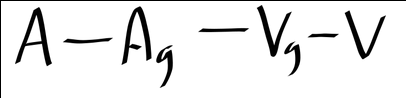
\includegraphics[width=0.5\textwidth]{basic}
\end{figure}
A basic attack which AITF is designed to combat is a simple flooding attack, as shown in figure [2]. In this scenario, the attacker “A” sends a large amount of data to the victim “V”. The AITF enabled routers Ag and Vg have attached their respective headers to the AITF shim layer. The victim determines if it is being attacked by keeping track of the number of packets it has received from each IP address per minute. If this number increases above a specified threshold, then this IP address is determined to be an attacker. 

As the policy controller, V decides that A is attacking him, and decides to issue a “please protect me”, or PPM packet to the first network in the shim stack, or Ag. A threeway handshake between V, Ag, and Vg occurs to verify that the PPM packet is coming from the source it is claiming to protect. The victim will send a packet containing an IP payload of a 64 bit nonce, and with the protocol field set to 253. Ag will intercept this packet and can verify two things: that the nonce is correct, and that the shim layers match (recall that Vg caches shim stacks by source IP). In the case that the nonces don’t match, Vg will escalate. In the case that the nonces match, but the shim layers do not match, Vg will escalate directly to the first matching layer in the shim stack. If both match, Vg will reply with the second nonce in the reply from Ag and ask Ag to filter traffic from A to V. If Ag cooperates, it will install a filter for T-long seconds to filter traffic between A and V. If Ag does not cooperate, then V will repeat this process, signifying that it wants an escalation. Vg will then attempt to have the gateway of Ag block traffic. 


\section{Escalation}
In the case that the attacker gateway or subsequent gateways do not comply, the request to block traffic will be escalated to gateways closer to the victim.  As the request gets escalated further and further, more traffic will be blocked.  Escalation is determined by an escalation policy implemented by the victim.  This policy ultimately chooses whether or not to escalate based on the benefit and cost of performing that escalation.  For this project, we will assume that escalation is always beneficial, and therefore escalation will always occur when an gateway does not comply.  This benefit comes from the assumption that most of the incoming traffic is from an attacker.  This will continue  up to the victim gateway and will ultimately disconnect the victim from the internet if no gateway complies with the filtering request.
Initially the victim gateway will put a filter for the attacking path in its TCAM memory.  It will then ask the attacker gateway to temporarily filter traffic on the attacking path.  At this point, the filter in the victim gateway’s TCAM memory will be moved to shadow memory.  If the victim receives a single packet from the attacker after initially complaining, the victim will send a request (“whine”) to the victim gateway communicating that it’s still receiving undesired flow.  This “whine” packet should be different than the original blocking request. This packet will make the IP protocol header 255  If the victim gateway receives a “whine” packet, it checks shadow memory to confirm that it already tried to resolve the issue with the attacker gateway.  The victim gateway will communicate to the attacker gateway to filter traffic to the victim.

\section{Spoofing Attacks and their Remediation}
Suppose that in figure [1], the attacker is actually Ag and the attacker is spoofing packets from H. Ag does this by falsifying a shim stack layer from Hg, before sending the packet to I, which will then sign it and pass it along to Vg. Assuming this traffic is detected as a malicious and V decides to block it, It will route back through Ag and I, before Hg will identify the packet as being spoofed. This is where the random number becomes important; Hg can tell detect a mismatch in hash function output and determine that it is spoofed. If this is the case; It will notify V of an attempted spoofing attack coming through router I, at which point V determines if it should escalate.

\section{Definitions}
\begin{description}
	\item[Shadow Memory] This is a slower form of memory than TCAM and is used to store information that does not need to be accessed in a timely manner
	\item[TCAM Memory] Ternary content-addressable memory (TCAM) is a type of high-speed memory that searches it’s contents in one clock cycle (similar to cache memory)
	\item[Attacking Path] The network path from the attacker to the victim
	\item[AITF] Active Internet Traffic Filtering
\end{description}

\section{Implementation}
\begin{enumerate}
	\item We will use a systems language, most likely C
	\item There will be a threshold for determining whether an attack is a DOS attack. This threshold will be kept in /etc/aitf.d/threshold.conf as a number of requests per IP per minute.
\end{enumerate}




\section{Assumptions}
\begin{enumerate}
	\item The victim and attacker are AITF enabled
	\item All end hosts are AITF enabled
	\item When a victim is being attacked, most incoming traffic is from an attacker. Therefore, escalation is always preferred over not escalating.
	\item Not all middle routers must be AITF enabled; however if a middle router is not AITF enabled, escalation may not occur TO that device, just over it.
\end{enumerate}

\end{document}